\newSec[Arch]{Clean Architecture}{1}



\newSec[ArchDepRule]{Dependency Rule}{2}

Wie in \refImg{fig:ArchPkg} zu sehen, zeigen alle Abhängigkeiten in die gleiche oder eine darunterliegende Schicht. Aufrufe werden mittels \textit{virtuellen} Klassen\footnote{\textit{virtuelle} Klassen in der Sprache c++ entsprechen \textit{abstrakten} Klassen in Java.} und einer entsprechenden \DepInv\ in weiter außen liegende Klassen ermöglicht.


\begin{figure}[ht!]
\vspace{0.25cm}
\begin{center}
\fbox{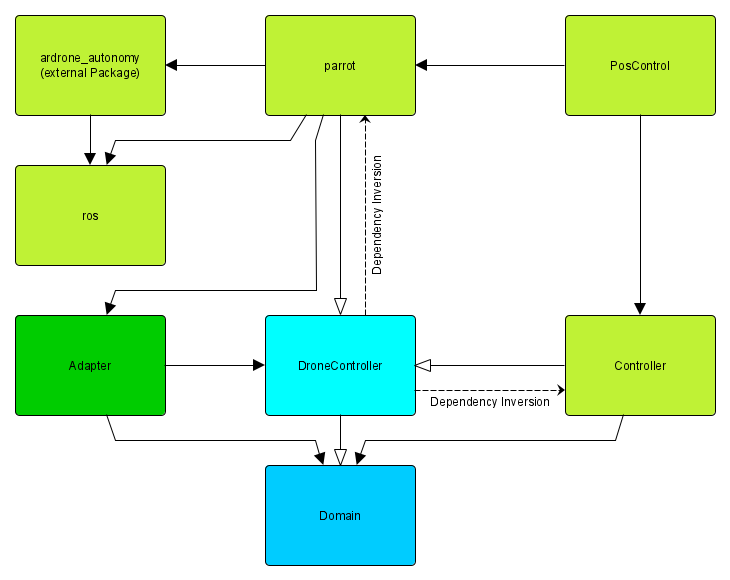
\includegraphics[width=15cm]{Pictures/Architecture Blocks.png}}
\caption{Architektur-Pakete des Projektes}
\label{fig:ArchPkg}
\end{center}

\vspace{0.25cm}
\href{https://github.com/MaagMich/SWE2\_Project/blob/c5c3674bd201ee306463881cf711bb2ce9229842/Ausarbeitung/Pictures/Architecture\%20Blocks.png}{Image-Link}\\
\refImgShort{fig:ArchPkg} zeigt das Konzept der Architektur. Die Bedeutungen der Pfeile orientieren sich an UML-Klassendiagrammen. Die Farbgebung unterscheidet die verschiedenen Schichten der \clean: \textit{Domain-Layer} (blau), \textit{Application-Layer} (hellblau), \textit{Adapter-Layer} (grün), \textit{PlugIn-Layer} (hellgrün).
\end{figure}



Ein detallierteres Verständnis der Interaktion der Klassen soll durch \refImg{fig:Arch} vermittelt werden.

\begin{figure}[ht!]
\vspace{0.25cm}
\begin{center}
\fbox{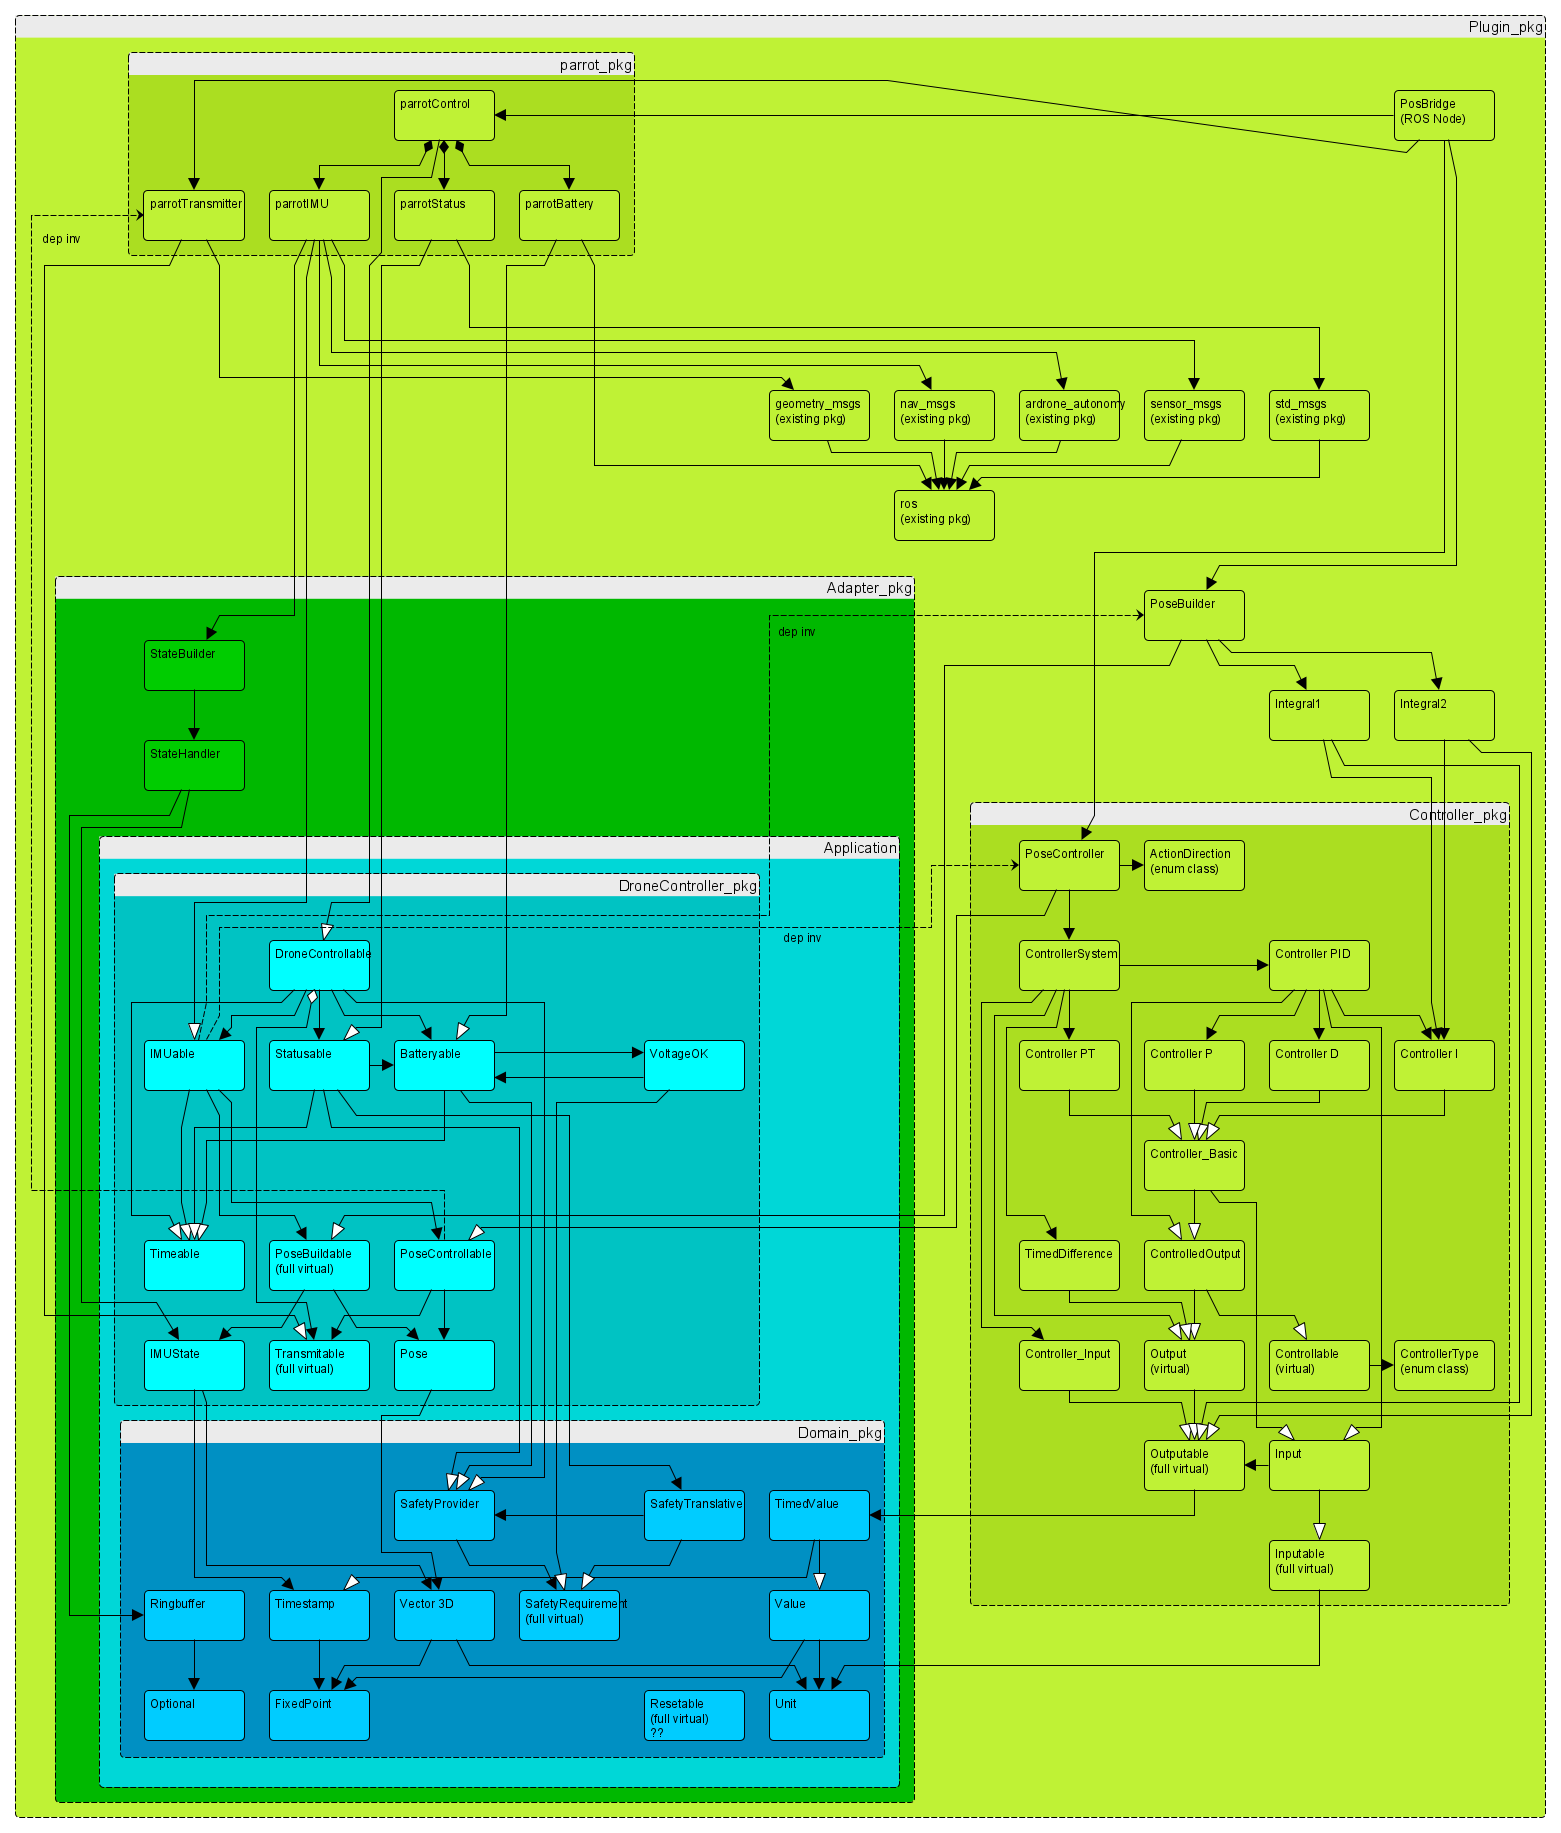
\includegraphics[width=15cm]{Pictures/Clean Architecture.png}}
\caption{Architektur des Projektes}
\label{fig:Arch}
\end{center}

\vspace{0.25cm}
\href{https://github.com/MaagMich/SWE2\_Project/blob/c5c3674bd201ee306463881cf711bb2ce9229842/Ausarbeitung/Pictures/Clean\%20Architecture.png}{Image-Link}
\end{figure}




\newSec[ArchDomain]{Domain Layer}{2}

Um ein Anlegen des \textit{Abstraction Layers} aus Angeberei zu vermeiden\footnote{Siehe Seite 23 in den Vorlesungsfolien zu \textit{Clean Architecture}}, wurden die beiden Schichten \textit{Abstraction Layer} und \textit{Domain Layer} vereinigt. Tatsächlich könnten folgende Klassen in einem \textit{Abstraction Layer} untergebracht werden:
\begin{itemize}
\item FixedPoint
\item Unit
\item Value
\item Vector3D
\item Timestamp
\item TimedValue 
\item Optional
\end{itemize}

Da die \CodeClass{SafetyRequirement}, \CodeClass{SafetyProvider} und \CodeClass{SafetyTranslative} den Use Case \texttt{\glqüberwacht einen sicheren Start \bzw\ Flug\grq} abbilden, sind diese Klassen entgegen der Aufteilung innerhalb des betrachteten Projekts dem \textit{Application Layer} zuzuordnen.



\newSec[ArchApp]{Application Layer}{2}
Der \textit{Application Layer} bildet eine \textit{Bridge} ab. Hierdurch kann die Hardware im zukünfigten Projektverlauf ausgetauscht werden, ohne den Kern der Anwendung zu beeinflussen.
Darüber hinaus bietet das \CodePkg{DroneController} die grundlegenden Funktionalitäten für die Positionsregelung einer Drohne an. Umfangreichere Funktionen, wie \zB\ die Kommunikation mit der Hardware, werden in dafür vorgesehenden Paket des \textit{PlugIn Layers} implementiert. 

Die \CodeClass{IMUState} und die \CodeClass{Pose} bilden Daten ab. Somit sind diese entgegen der Darstellung in \refImg{fig:Arch} dem \textit{Domain Layer} zugehörig.



\newSec[ArchAdapter]{Adapter Layer}{2}
Die \CodeClass{StateBuilder} ermöglicht eine Transformation der Informationen der \textit{IMU-Message} in die dafür vorgesehene \CodeClass{IMUState}. Die entstehende Instanz wird anschließend zur weiteren Verarbeitung in die Implementierung der Klasse \CodeClass{PoseBuildable} übergeben.



\newSec[ArchPlugin]{PlugIn Layer}{2}
Das Framework \ROS\ wurde gezielt in den \textit{PlugIn Layer} aufgenommen, um etwaigen Änderunges dieses Frameworks mit mäßigem Aufwand begegnen zu können.
\note{\glqq The Robot Operating System (ROS) is a set of software libraries and tools that help you build robot applications. From drivers to state-of-the-art algorithms, and with powerful developer tools, ROS has what you need for your next robotics project. And it's all open source.\grqq\cite{ROS}}

Des Weiteren wird die vollständige Implementierung der einzusetztenden Drohne, sowie des Controllers im \textit{PlugIn Layer} geführt. Somit ist ein einfacher Austausch möglich.

\newSec[ArchPluginMain]{main() Methode}{4}
Die \CodeMeth{main()} hat die Aufgabe, die Applikation als Ganzes zusammenzusetzen. Sie muss im \textit{PlugIn Layer} angesiedelt sein, um für das initialisierten des Programms Zugriff auf alle PlugIns zu haben.
Im Code wird in der \CodeMeth{main()} eine Instanz der \CodeClass{MainClass} instanziiert, welche die eigentliche Aufgabe der \CodeMeth{main()} übernimmt (vgl. \refImg{fig:Arch}). Anschließend wird in der \CodeMeth{main()} die Fluss-Steuerung des \ROS-Eventbusses realisiert (\href{https://github.com/MobMonRob/ROSLabDrohne/blob/603d50c276cbb1a44929cd096f8a4dc1ce6df855/Code/PosControl/src/Main.cpp\#L15}{Link: while(ros::ok()) spinOnce()}).










